\documentclass[11pt]{article}
\usepackage{scicite}
\usepackage[utf8]{inputenc}

% Default packages
\usepackage{amsmath, amsfonts, amssymb, amsthm, epsfig, epstopdf, titling, url, array}
\usepackage{algorithm} 
\usepackage{algorithmic} 
\usepackage{graphicx}
% Because it is convenient
\usepackage{hyperref}

% To insert tables
\usepackage{array}

% We might need some code insertion
\usepackage{minted}

% Also indent first paragraph of a section
\usepackage{indentfirst}


\theoremstyle{plain}
\newtheorem{thm}{Theorem}[section]
\newtheorem{lem}[thm]{Lemma}
\newtheorem{prop}[thm]{Proposition}
\newtheorem*{cor}{Corollary}

\theoremstyle{definition}
\newtheorem{defn}{Definition}[section]
\newtheorem{conj}{Conjecture}[section]
\newtheorem{exmp}{Example}[section]

\theoremstyle{remark}
\newtheorem*{rem}{Remark}
\newtheorem*{note}{Note}



\topmargin 0.0cm
\oddsidemargin 0.2cm
\textwidth 16cm 
\textheight 21cm
\footskip 1.0cm

\newenvironment{sciabstract}{
\begin{quote} \bf}
{\end{quote}}
\renewcommand\refname{References and Notes}

\newcounter{lastnote}
\newenvironment{scilastnote}{\setcounter{lastnote}{\value{enumiv}}
\addtocounter{lastnote}{+1}
\begin{list}
  {\arabic{lastnote}.}
  {\setlength{\leftmargin}{.22in}}
  {\setlength{\labelsep}{.5em}}}
{\end{list}}


% Include your paper's title here

\title{Wikipedia Recommender System with serendipity} 


\author
    {
      Barszezak Yoann, Bricout Rapha\"el, David Nicolas, Dupr\'e R\'emi,\\
      Fouch\'e Aziz, Gourdel Garance, Kaddar Younesse, Mallem Maher,\\
      \\
      \normalsize{Department of Computer science, ENS Paris-Saclay}\\
    }

 

    \date{November 2017}



%%%%%%%%%%%%%%%%% END OF PREAMBLE %%%%%%%%%%%%%%%%



\begin{document} 

% Double-space the manuscript.

\baselineskip10pt

% Make the title.

\maketitle 



% Place your abstract within the special {sciabstract} environment.

\begin{sciabstract}
  TO DO : Abstract\\
  Younesse : Github -> Overleaf sync test\\
  Younesse : Overleaf -> Github sync test
\end{sciabstract}


\tableofcontents


\section*{Introduction}

Since a few decades, recommender systems have been everywhere ; from audiovisual services like \textit{YouTube} or \textit{Deezer} with the \textit{"Flow"}, to market platforms like \textit{Amazon}, or through apps stores or even web browsers, about everyone uses at least one of them every day. 

They usually consist in algorithms that, given user previous selections (content streamed, words searched or items bought), try to guess which content is likely to be selected by the user next. \\

With statistical learning comes a natural approach to this problem : for each user \textit{John}, the system aims to train a model which tends to fit the user tastes, to be able to deliver good predictions. One of the easiest and most natural way to apply that is to find the users whose tastes are the closest to \textit{John}'s ones. Then, by simply watching at their advice on an asked product, this is easy to get an idea about how it will be likely to be appreciated by \textit{John}.

Unfortunately, there are many limitations in this method. The main one is that, if there are not enough users in the system, and if there are many objects to rate, the intersection between users ratings is the empty set with a high probability. Furthermore, tastes are evolving ; if an user has given a music five stars ten years ago, then there is no reason he still likes it that much. Finally, this approach implies to be able to define a metric on ratable objects, which can sometimes be very difficult, or even poorly relevant. \\

Reinforcement learning with deep neural networks can overcome these drawbacks, by drastically moving the focal. Instead of starting from a state of the system where many users have already given their ratings, it can be beneficial to start from zero for each user, then start building the model depending on his feedbacks. The system gives a new user a first proposition, and according to his advice on this proposition (\textit{I like/I am not interested}, the model proposes him more and more suggestions trying to fit more and more its tastes, trying to get more \textit{I like} which can be seen as the reward of the experience. Of course, the more active the user is the more accurate tends to be the prediction. \\

One of the big questions which has been to be faced has been : To which data set will be applied this theory ? We finally converged to the biggest collaborative encyclopedia all over the world. \\

\textit{Wikipedia} is huge. Only considering English-written articles, there are more than 5,000,000 of pages, describing hundreds of themes. According to official statistics, 600 brand new articles are published each day. In one hand, these values mean a gigantic amount of knowledge within easy reach, but in the other hand the platform gets all the drawbacks of a collaborative system : fake news, vandalism, incomplete articles... 

Even for an experienced user, browsing this mass of data may be hazardous : whereas searching for a precise page works very well, finding new topics connected to subjects the user used to be interested in can be tough. This wanting is called \textit{serendipity}. 

\begin{center}
\textbf{Definition, Serendipity}}, \textit{serendipity means a "fortunate happenstance" or "pleasant surprise". }
\end{center}


todo goal of the web extension

\section{Problem Overview}
-Wikipedia
-recommander system
-serendipity (def)
-questions : like/dislike, specific/general
-NN
-Implementation
(at least)



\section{Retrieval of Candidate articles}

\subsection{Neighborhood}

Let's try to understand the idea of proximity between two articles. One way to do it is to introduce a potential function telling us the proximity between two articles.

\subsubsection{Naive Similarity}

Our attempt to define this potential function uses the set of categories linked to an article, it is called the similarity.





\vspace*{5mm}
\begin{defn}
  Let $a_1$ and $a_2$ be two articles. We call $C_1$ (resp. $C_2$) the set of categories linked to $a_1$ (resp. $a_2$).
  We define the similarity of $a_1$ and $a_2$ the following quantity:\\
  \begin{equation*}
    S_W(a_1,a_2) = \frac{Card(C_1 \cap C_2)}{min(Card(C_1),Card(C_2))}
  \end{equation*}
\end{defn}

\begin{rem}
  $\forall a_1\: a_2,\; S_W(a_1,a_2) \in [0,1]$
\end{rem}

\vspace*{5mm}
With this definition in mind, let's seek for an output of the ``Retrieval of Candidate Articles''.


Let's call $a_c$ the current article.
Given an subinterval $I$ of $[0,1]$ (define in the serendipity subsection), one way to find candidate articles will be to pick randomly $N$ articles $(a_i)_{1 \leq i \leq N}$ such that:
\begin{center}
  $\forall i \; S_W(a_c,a_i) \in I$
\end{center}

\vspace*{5mm}
This approach should work as long as the similarity is precise (in the case of Wikipedia, it means as long as an article have a significant number of categories). Unfortunately, some articles are poorly categorized. Thus, it is not always accurate to use this object.\\
Therefore, an other approach is needed.






\subsubsection{Ontology basis}

An other way to solve this problem is to use an Ontology on the Wikipedia articles.

\vspace*{5mm}
\begin{defn}
  Let $A$ a set of theme. We call $\mathbb{O}$ an Ontology over $A$ a directed tree in which :
  \begin{itemize}
  \item $ Node(\mathbb{O}) = A$
  \item if $t_1$ is a sub-theme of $t_2$ then $(t_1,t_2) \in Edge(\mathbb{O})$
  \end{itemize}
\end{defn}

\vspace*{5mm}

\begin{rem}
  The relation ``is a sub-theme'' is not transitive.
\end{rem}

\begin{figure}[!h]
	\centering
    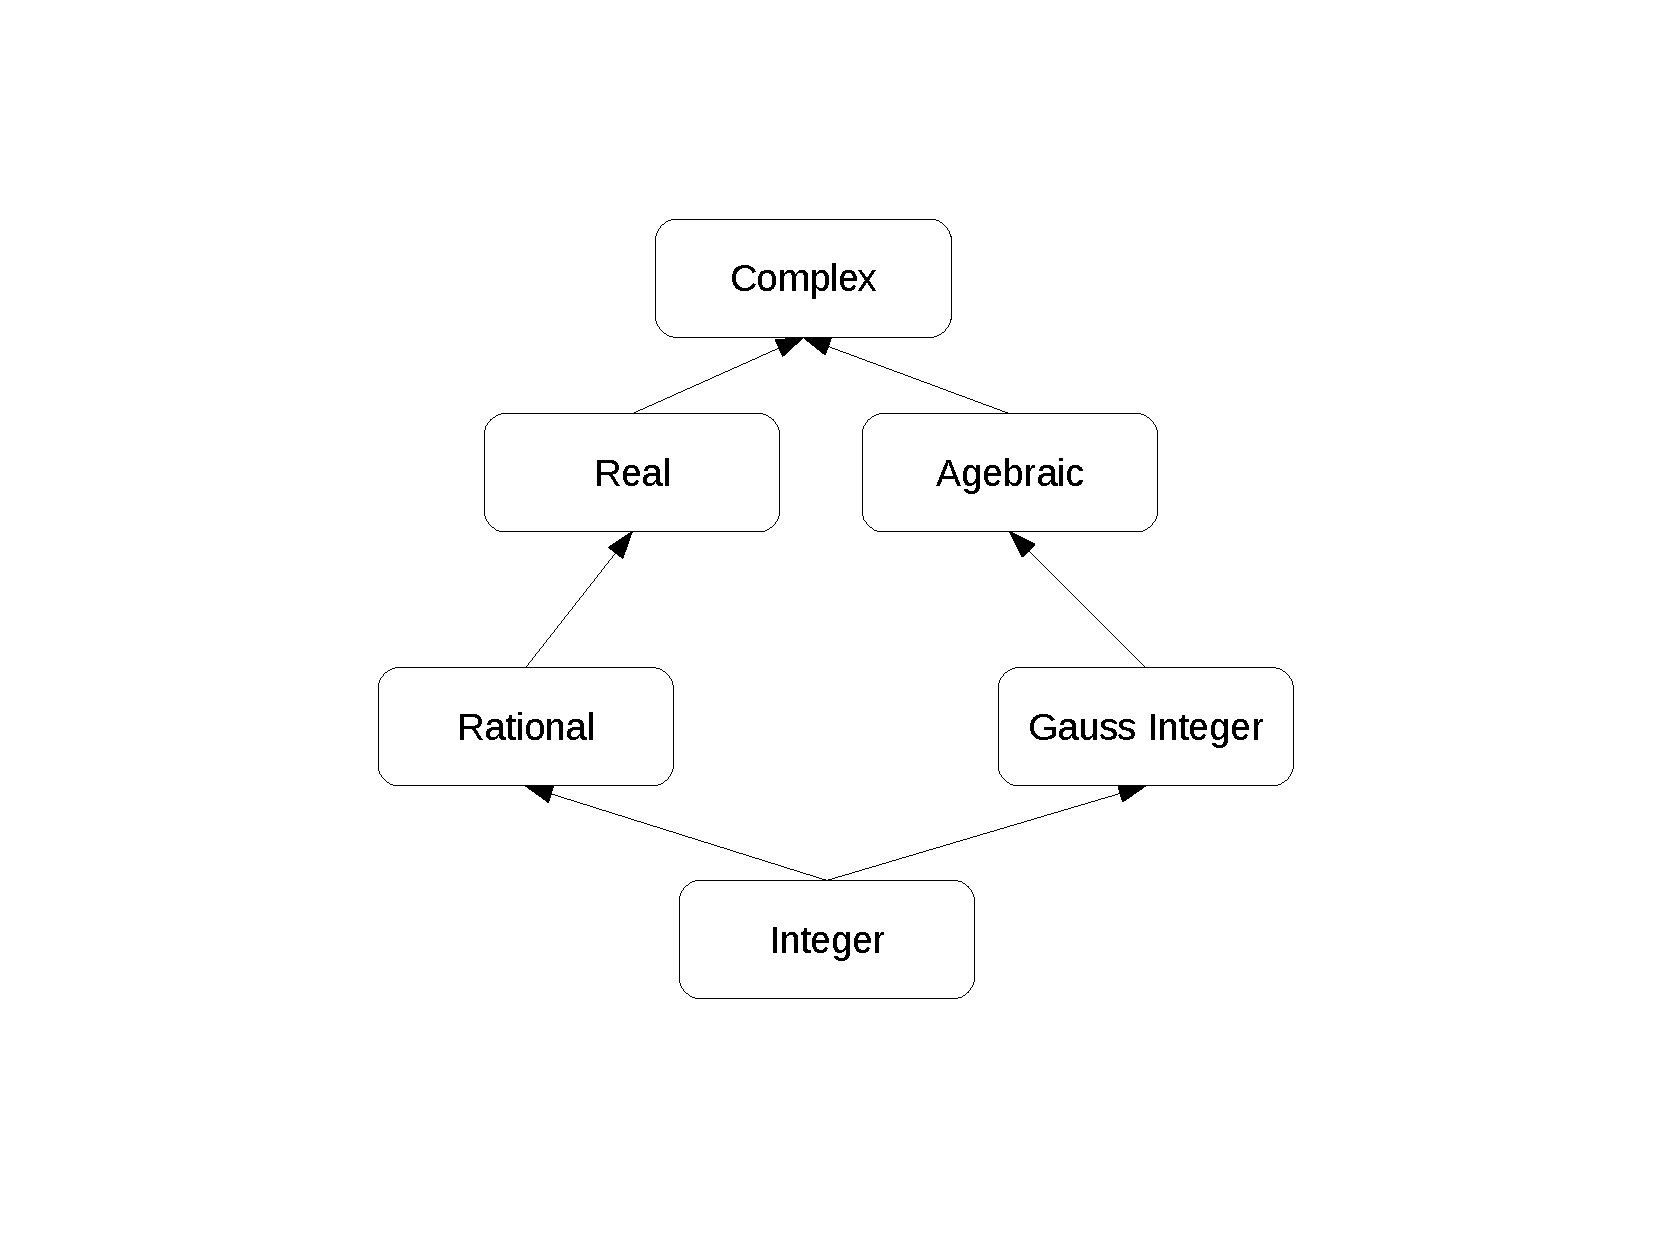
\includegraphics[scale = 0.3]{ExOntology.pdf}
    \caption{Ontology over number}
\end{figure}

This kind of structure is available on a YAGO software (Yet An Other Great Ontology). Thus, the building of such an ontology on Wikipedia is not required. In the following, we will suppose that every theme in YAGO matches with an article on Wikipedia. \\
Now that we have in mind the definition of ontology, let's try to find a way of using it to select articles.\\


\begin{algorithm}
  \caption{Calculate $A^*$ the selected articles}
  \begin{algorithmic}
    \REQUIRE $wish \in \{specific , general\}$ , $p_1 \: ,p_2 \in ]0,1[ $, $N \in \mathbb{N}$ , $a_c \in A$
    \STATE $A^* \leftarrow \emptyset$
    \WHILE {$ Card(A) \leq N $}
    \IF {$wish = specific$}
    \STATE $ r \leftarrow geometric.random(p_1)$
    \STATE Ask YAGO a for a random son of depth r from $a_c$
    \STATE $ A^* \leftarrow A^* \cup \{a_{YAGO}\}$
    \ELSE
    \STATE $ r \leftarrow geometric.random(p_2)$
    \STATE Ask YAGO a for a random father of depth r from $a_c$
    \STATE $ A^*  \leftarrow A^* \cup \{a_{YAGO}\}$ 
    \ENDIF
    \ENDWHILE
    \RETURN $A^*$
  \end{algorithmic}
\end{algorithm}

-choix de p1 et p2 dans serendipity

\newpage
\subsection{serendipity}
\subsection{Serendipity}

In the previous algorithm, the set of candidate articles was chosen among the nearest neighbors in the ontology of YAGO.
In order to recommand to the user articles far from its habits, we present here another way to find articles, depending on the 'serendipity' factor I.
\begin{algorithm}
  \caption{Calculate $A^*$ the selected articles}
  \begin{algorithmic}
    \REQUIRE $wish \in \{specific , general\}$ , $N \in \mathbb{N}$, $c \in \mathbb{N}$, $a_c\in A$
    \STATE $A^* \leftarrow \emptyset$
    \WHILE {$Card(A^*)\leq N$}
    \WHILE {$Card(Cat_{YAGO}(a))\leq c$}
    \STATE Ask YAGO for a random father of a in YAGO 
    \STATE $a \leftarrow a_{YAGO}$ 
    \ENDWHILE
    \STATE $a^* \leftarrow rand.article(A\setminus A_{visited})$
    \WHILE {$S_W(a^*,a)\notin I$}
    \STATE $a^*\leftarrow rand.article(A\setminus A_{visited})$
    \ENDWHILE
    \STATE $ A^* \leftarrow A^* \cup \{a_{YAGO}\}$
    \ENDWHILE
    \RETURN $A^*$
  \end{algorithmic}
\end{algorithm}

-serendipity in our recommander system (button : how to use it ?)
-algorithm for the choice of 'serendipity (How to chose I ?)
\subsubsection{Similarity}

-choice of I


\section{Candidate Ranking}

\subsection{possible input in neural network}

\subsubsection{Category vector}

One of the very accessible tool to analyze a wikipedia page is(, as we mentioned ?), the use of the categories assigned to each page that can be obtained through the Wikipedia API.
Only looking at some often viewed wikipedia page, would have us thinking that those categories can act as key word for the article. For example the Michael Jackson wikipedia page has almost a hundred categories, quite diverse :
 \begin{center}
	\texttt{"21st-century American singers" "Accidental deaths in California" "African-American choreographers" "African-American rock singers" "African-American songwriters"  "People acquitted of sex crimes"}
 \end{center}

Nevertheless you would also notice that they are some less relevant categories. The first categories regard the page itself, it's link, it's sources, or even some precise month since it needs clarification.

 \begin{center}
	\texttt{"All articles with dead external links" "CS1 Spanish-language sources (es)" "Articles with dead external links from July 2013" "Wikipedia articles needing clarification from January 2017"}
 \end{center}
But an issue with this strategy may be that some very specific article won't be descripte precisly enough with there category 


Categories of the wikipedia page "functors" (in theory of category)
"Pages using web citations with no URL","Functors","Mathematics navigational boxes"

\subsubsection{Word2Vect and Wikidata}

\subsection{Wide and deep Neural Network}
\subsubsection{Wide : memorization/focus}
\subsubsection{Deep : generalization/serendipity}


\newpage

\section{System architecture}

First, we give a global diagram to expose interactions between the user interface, \textit{Wikipedia} pages, modules and \textit{Wikipedia} APIs. 

\begin{figure}[h!]
	\centering
    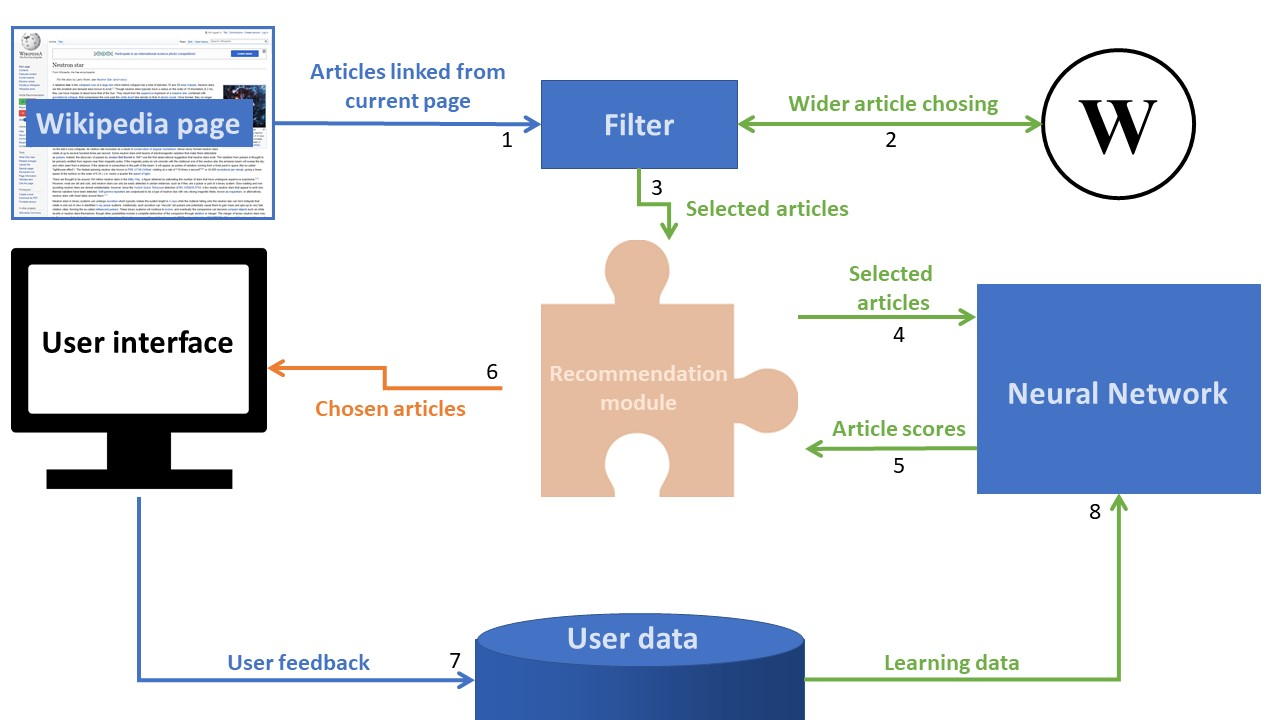
\includegraphics[width=400pt]{diagram.png}
    \caption{Global software's structure}
    \label{arch_glo}
\end{figure}

Blue arrows represent system's input, orange arrow is for the output. Green arrows explains how data is exchanged internally between the different modules. Arrowed labeling is defined as follows :
\begin{itemize}
\item \textbf{1)} \textit{Extraction of all links mentioned in the article (without the links of header, side, and footer)}.
\item \textbf{2)} \textit{Visit of article neighborhood (it may be 2-hop neighboring) to enhance serendipity, selection of best neighbors based on general criteria}.
\item \textbf{3)} \textit{Selected articles are injected into the recommendation module}.
\item \textbf{4), 5)} \textit{Recommendation module feeds the user-specific neural network with selected articles to sort them}.
\item \textbf{6)} \textit{Best articles are re-injected into the page, to be recommended to the user}.
\item \textbf{7)} \textit{User gives its feedback on proposed articles, reactions are stored locally}.
\item \textbf{8)} \textit{Thanks to user feedback, network structure is updated to fit user's interests}.
\end{itemize}

\subsection{Zoom on recommendation method}

\begin{figure}[h!]
	\centering
    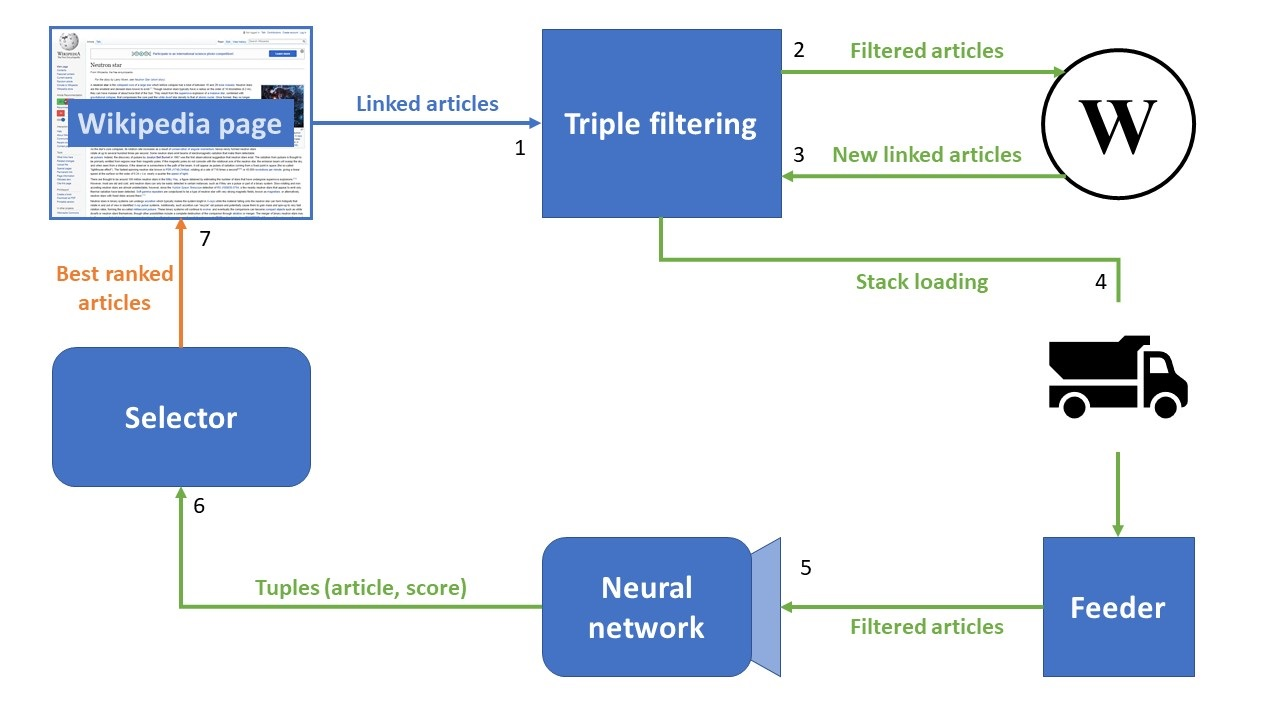
\includegraphics[width=400pt]{diagram_zoom.png}
    \caption{How recommendation method works}
    \label{arch_glo}
\end{figure}

\subsubsection{Triple filtering}

The main challenge which has been to be faced is the HTTP requests' efficiency problem. Indeed, the first idea is to get all page links, visit them all and sort them using some pertinence criteria. It was nevertheless technically impossible ; due to the size of HTTP requests, even performed asynchronously, the answer time was huge. \\

The solution developed was to introduce a triple filtering, which consists in three passes going more and more complex and time-expensive, but on less and less entries. It allowed the module to be able to explore pages to \textit{2-hops} from the original page

\begin{itemize}
\item \textit{Title-based filtering} With syntactically simple regular expressions, we can describe the set of hyper links that must be irrelevant. For instance there are years, ISBN codes, image links... All of them can be thrown away without even accessing their HTTP content.
\item \textit{Popularity-based filtering} In a second time, a probabilistic model has been introduced whose the purpose has been to determine how likely a page was to be liked by the user. \textit{Wikipedia}, through its \textit{API} called \textit{Wikimedia} allows, with a simple HTTP request weighting only a few dozens of characters, to access the views count of a certain page for a certain time lapse. Using it, one can identify connected trending content the user must be interested in.
\item {Content-based filtering} Finally, the module does its last selection by focusing on articles content. This part is the most expensive, as it is necessary to get the full page content for each remaining article, and to analyze it. This time, one focus on incomplete articles or poorly written (articles containing only a few words for example). \textit{This part could clearly be improved by a deeper text analysis, and probably get way better results.}
\end{itemize}

\subsubsection{Feeder and selector}

Feeder and selector manage neural network's input and output. Feeder gathers last filter output, then vectorizes it by applying the following operation ; 

\subsubsection{Neural network and learning}

\subsection{User interface}
We started the implementation of an in-browser plugin for Wikipedia suggestion.
The goal of this plugin is to insert an interface in any Wikipedia page that allows the user to give his opinion about this page. The plugin will keep an user profile up to date and suggest Wikipedia pages to the user that it considers relevant for this user.

As our goal is to introduce serendipity in such a system, we also added a cursor to parametrize a level of serendipity. Bigger this parameter is set, the less the user will be suggested pages about a topic he already eared of.

\subsection{Wikipedia API's}
% a few words about what both api provide


\section{Experimentation}
\subsection{Similarity}
Using Wikipedia official api, we were able to calculate the naive similarity between two pages defined at \ref{definition:S_w}. For example, the following code will prompt $0.6364$, the similarity processed between the page about Jimi Hendrix (of id 16095) and Michael Jackson (of id 14995351).
  \mint{javascript}|apiMod.distance(16095, 14995351, console.log); // "similarity(Michael J.,  Jimi H.)"|
  
Thus, we were able to experiment this distance over a set of web pages. We can thus qualitatively test this algorithm. It is not really hard to get examples where this calculation is irrelevant (for example, Michael Jackson is closer to France than Paris, cf. Figure \ref{fig:similarity}), but still, on many examples, it gives a trend that fits with the intuition.

\begin{figure}
    \caption{Comparison of some pages of Wikipedia (cf definition \ref{definition:S_w})}
    \label{fig:similarity}
	\centering
	\begin{tabular}{c|c|c}
		Page 1			&	Page 2			&	Similarity \\
		\hline\hline
		Michael Jackson	&	Jimi Hendrix	&	0.6364	\\
		Michael Jackson	&	France			&	0.8600	\\
		Paris			&	France			&	0.6842	\\
		Luxembourg		&	France			&	0.5416	\\
  \end{tabular}
\end{figure}


\section{State of the Art}



\bibliography{scibib}

\bibliographystyle{Science}

\end{document}
